\clearpage
\twocolumn[{%
\rqparent
\subsection{Decision accuracy on decisive pairs}
\label{app:rq02_decisive_pairs}

\noindent\begin{minipage}[t]{0.485\textwidth}
\vspace{0pt}
\paragraph{Research Question.} \emph{Does a proxy rank the design decisions better once the pairs the 1.7B reference itself cannot separate from seed noise are left out?}

\paragraph{Setup.} We measure DA-size on the pairs that the 1.7B reference separates by more than seed noise. We use the seed-1904 runs of every language setting, ladder and data build. The proxies (90M--1B) are compared against the final 1.7B checkpoint, on pairs that differ on any number of design axes. A pair is decisive for a task when its 1.7B gap exceeds k √2 times the task's seed standard deviation, for k $\in$ \{1, 2\}. The factor √2 turns the noise of one run into the noise of a difference of two runs. A task's seed standard deviation is the standard deviation of its final score across seeds, taken as the median over the replicated baseline cells (175M, 600M and 1B). There are no replicates at 1.7B, so the threshold assumes that seed noise does not grow with size. Every line reads the same tasks: the benchmark tasks and their bBPB twins with a seed standard deviation and at least three decisive pairs at k = 2, above chance at the proxy and at 1.7B, and the per-language BPB of the 50 trained languages. Each line divides the matching pairs by the comparable pairs, summed over tasks, so a task weighs by its pairs: on BPB English holds 17 \% of the decisive pairs at k = 2, and the mean over the 50 languages is higher at 600M (0.99 against 0.95, \texttt{da\_cell\_mean} in the CSV, as in the definition table of the DA appendix).
\end{minipage}\hfill
\begin{minipage}[t]{0.485\textwidth}
\vspace{0pt}
\begin{rqfinding}
\textbf{1. Benchmark DA rises on decisive pairs.} On the same 876--1020 tasks, multi-axis DA-size goes from 0.58--0.59 on every pair to 0.64--0.66 above one seed sd and 0.71--0.73 above two, so part of the gap to 1 is the reference's own noise and not the proxy's. (Figure~\ref{fig:app_rq02_decisive_pairs}.)
\\
\\
\textbf{2. Most benchmark pairs are not decisive.} One seed sd keeps 52--53 \% of the comparable pairs and two keep 25 \%, so on a single benchmark task the reference separates few of the design pairs.
\\
\\
\textbf{3. BPB is near perfect on decisive pairs.} It reads 0.89--0.98 above one seed sd and 0.95--0.995 above two, with 72 \% and 52 \% of the pairs kept.
\end{rqfinding}
\end{minipage}

\vspace{\baselineskip}
\noindent\begin{minipage}{\textwidth}
\centering
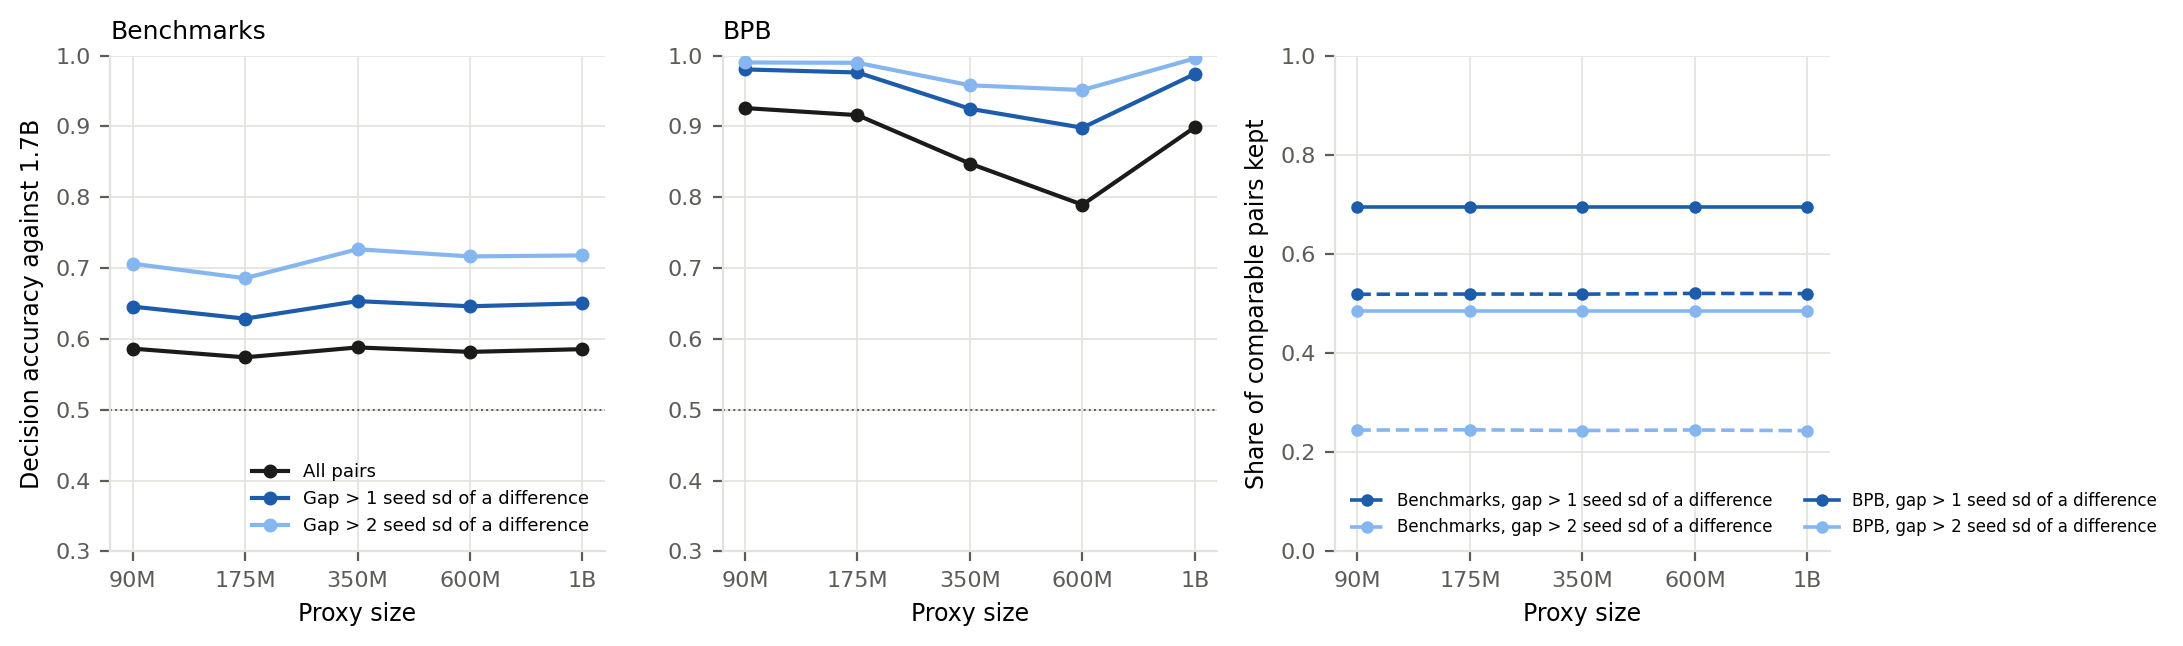
\includegraphics[width=\textwidth,height=0.36\textheight,keepaspectratio]{figures/app_rq02_decisive_pairs.png}
% source: src/signal-and-noise/analysis/rq02_decisive_pairs/pretraining/predictivity/decisive_pairs_da_size_paper.png
\captionof{figure}{\textbf{Benchmark DA rises on decisive pairs.} DA-size of the final checkpoint of each proxy size against the 1.7B final checkpoint, on multi-axis design pairs, pooled over decisions, for the benchmark tasks with their bBPB twins (left) and the per-language bits per byte (middle). One line per threshold: every comparable pair (black) and the pairs whose 1.7B gap exceeds one or two seed standard deviations of a difference (dark and light blue). The dotted line marks 0.5. Right: the share of the comparable pairs each threshold keeps, solid for the bits per byte and dashed for the benchmarks.}
\label{fig:app_rq02_decisive_pairs}
\end{minipage}
}]
